\documentclass[a4paper,11pt]{article}

\usepackage{amsmath,amssymb, amsthm}
\usepackage{charter}
%\usepackage{calc}

\usepackage{fullpage}

\usepackage{multirow}
%\usepackage[cp1250]{inputenc}
%\usepackage[T1]{fontenc}
%\usepackage{calligra}
%\usepackage[slovak]{babel}
\usepackage{amsfonts}
\usepackage{layout}
\usepackage[dvips]{graphicx}
\usepackage{url}
\usepackage{color}
\usepackage{graphicx}
\usepackage{algorithmic}
\usepackage{algorithm}
\usepackage{verbatim}
\usepackage{epsfig}
\usepackage[colorlinks,
            linkcolor=red,
            anchorcolor=blue,
            citecolor=blue
            ]{hyperref}
\usepackage{xcolor}

\renewcommand{\algorithmicrequire}{\textbf{Input:}}
\renewcommand{\algorithmicensure}{\textbf{Output:}}

\newcommand{\hlight}[2]{\noindent\colorbox{#1}{%
    \parbox{\dimexpr\linewidth-1\fboxsep}% a box with line-breaks that's just wide enough
        {#2%
        }}}

\newcommand{\HRule}{\rule{\linewidth}{0.5mm}}
 \newcommand{\xtilde}{\tilde x}
 \newcommand{\vtilde}{\tilde v}
 \newcommand{\Embb}{\E}
 \newcommand{\xbar}{\bar x}
 \newcommand{\ie}{\textit{i.e.}}
 
\newcommand{\main}[1]{\footnotesize\textbf{#1}} 
\newcommand{\todo}[1]{{\color{red}#1}}
\newcommand\tagthis{\addtocounter{equation}{1}\tag{\theequation}}


\newcommand{\del}[1]{{\color{red}#1}}

\let\la=\langle
\let\ra=\rangle

\newcommand{\st}{\;:\;}
\newcommand{\ve}[2]{\langle #1 ,  #2 \rangle}

\newcommand{\eqdef}{\stackrel{\text{def}}{=}}

\newcommand{\ii}{{}^{(i)}}

\newcommand{\R}{\mathbb{R}}
\newcommand{\Prob}{\mathbf{Prob}}
\newcommand{\E}{\mathbb{E}}
\newcommand{\Q}{\mathbb{Q}}
\newcommand{\Z}{\mathbb{Z}}

\newcommand{\vc}[2]{#1^{(#2)}}
\newcommand{\nc}[2]{{\color{red}\|#1\|_{(#2)}}}
\newcommand{\ncs}[2]{\|#1\|^2_{(#2)}}
\newcommand{\ncc}[2]{{\color{red}\|#1\|^*_{(#2)}}}
\newcommand{\ls}[1]{{\color{red} \mathcal S(#1)}}
\newcommand{\Rw}[2]{\mathcal R_{#1}(#2)}
\newcommand{\Rws}[2]{\mathcal R^2_{#1}(#2)}
\newcommand{\m}[1]{~\mbox{#1}~}

\newcommand{\nbp}[2]{\|#1\|_{(#2)}}   % norm block primal
\newcommand{\nbd}[2]{\|#1\|_{(#2)}^*} % norm block dual

\newcommand{\lf}{\mathcal L}
\newcommand{\U}{U}
\newcommand{\N}{N}
\newcommand{\mc}[1]{\mathcal #1}

\newcommand{\mLi}{{\color{red}m^{(i)}}}
\newcommand{\gLi}{{\color{red}g^{(i)}}}
%\newcommand{\TLi}{{\color{red}T_L^{(i)}}}
\newcommand{\TLi}[1]{{\color{blue}T^{(#1)}}}

\newcommand{\Lip}{L}

\newcommand{\Rc}[1]{{\color{red}  \mathbf{RC}_{(#1)}}}
\newcommand{\NRCDM}{{\color{red}NRCDM}\  }
\newcommand{\nnz}[1]{{\color{red}\|#1\|_0}}
% sets
\DeclareMathOperator{\card}{card}       % cardinality of a set
\DeclareMathOperator{\diam}{diam}       % diameter of a set
\DeclareMathOperator{\MVEE}{MVEE}       % minim volume enclosing ellipsoid of a set
\DeclareMathOperator{\vol}{vol}         % volume of a set

\DeclareMathOperator{\prox}{prox}         

% statistical
\DeclareMathOperator{\Exp}{\mathbf{E}}           % expectation
\DeclareMathOperator{\Cov}{Cov}         % covariance
\DeclareMathOperator{\Var}{Var}         % variance
\DeclareMathOperator{\Corr}{Corr}       % correlation

% functions and operators
\DeclareMathOperator{\signum}{sign}     % signum/sign of a scalar
\DeclareMathOperator{\dom}{dom}         % domain
\DeclareMathOperator{\epi}{epi}         % epigraph
\DeclareMathOperator{\Ker}{null}        % nullspace/kernel
\DeclareMathOperator{\nullspace}{null}  % nullpsace
\DeclareMathOperator{\range}{range}     % range
\DeclareMathOperator{\Image}{Im}        % image
\DeclareMathOperator{\argmin}{argmin}        % argmin

% topology
\DeclareMathOperator{\interior}{int}    % interior
\DeclareMathOperator{\ri}{rint}         % relative interior
\DeclareMathOperator{\rint}{rint}       % relative interior
\DeclareMathOperator{\bdry}{bdry}       % boundary
\DeclareMathOperator{\cl}{cl}           % closure

% vectors, matrices
\DeclareMathOperator{\linspan}{span}
\DeclareMathOperator{\linspace}{linspace}
\DeclareMathOperator{\cone}{cone}

\DeclareMathOperator{\tr}{tr}           % trace
\DeclareMathOperator{\rank}{rank}       % rank
\DeclareMathOperator{\conv}{conv}       % convex hull
\DeclareMathOperator{\Diag}{Diag}       % Diag(v) = diagonal matrix with v_i on the diagonal
\DeclareMathOperator{\diag}{diag}       % diag(D) = the diagonal vector of matrix D

\DeclareMathOperator{\Arg}{Arg}         % Argument

%\renewcommand{\qedsymbol}{\ding{114}}


\newtheorem{assumption}{Assumption}
\newtheorem{lemma}{Lemma}
\newtheorem{algorithms}{Algorithm}
\newtheorem{theorem}{Theorem}
\newtheorem{proposition}{Proposition}
\newtheorem{example}{Example}
\newtheorem{remark}{Remark}

\theoremstyle{plain}

\newtheorem{prop}[theorem]{Proposition}
\newtheorem{cor}[theorem]{Corollary}
\newtheorem{lem}[theorem]{Lemma}
\newtheorem{claim}[theorem]{Claim}
%\newtheorem{remark}[theorem]{Remark}

\theoremstyle{definition}

\newtheorem{exercise}[theorem]{Exercise}

\newtheorem{rem}[theorem]{Remark}
\newtheorem{que}[theorem]{Question}
\newtheorem{definition}[theorem]{Definition}

 
\begin{document}

\begin{titlepage}
\begin{center}

% Upper part of the page. The '~' is needed because \\
% only works if a paragraph has started.


\includegraphics[width=0.15\textwidth]{lehigh.jpg}~\\[1cm]

\textsc{\LARGE Lehigh University}\\[1.5cm]

\textsc{\Large 418 Final Project}\\[0.5cm]

% Title
\HRule \\[0.4cm]
{ \Large \bfseries On the exact separation of mixed integer knapsack cuts\\[0.4cm] }
%{ \small \bfseries Based on \cite{csizmadia2012s} and some related papers \\[0.4cm] }

\HRule \\[1.5cm]

% Author and supervisor
\noindent
\begin{minipage}{0.4\textwidth}
\begin{flushleft} \large
\emph{Author:}\\
Chenxin Ma, Xi He
\end{flushleft}
\end{minipage}%
\begin{minipage}{0.4\textwidth}
\begin{flushright} \large
\emph{Supervisor:} \\
Prof.~Ted Ralphs
\end{flushright}
\end{minipage}

\vfill

% Bottom of the page
{\Large Fall 2014}

\end{center}
\end{titlepage}

\tableofcontents
\newpage

\section{Introduction} 
Consider a positive integer $n$, letting $b\in\Q$, $a\in \Q^n$, $l\in \{\Q\cup \{-\infty\}\}^n$, $u\in \{\Q\cup \{+\infty\}\}^n$ and $I\subset [n] :=
\{1,...,n\}$. The Mixed Integer Knapsack Set is defined as
\begin{equation}\label{K}
 K=\{x\in \R^n : a^Tx\leq b, l\leq x\leq u, x_i\in \Z, \forall i\in I\}.
\end{equation}

Furthermore, if we have $c\in \Q^n$ and assume $l_i$ is finite for each $i\in [n]$, then the Mixed Integer Knapsack Problem (MIKP) can be 
described as:
\begin{equation}\label{MIKP}
 \max \{c^Tx:x\in K\}.
\end{equation}

We assume that for each $k=1,2,\dots,n$ either $a_k\neq 0$ or $c_k\neq 0$, otherwise, we could remove variable $x_k$ without affecting the problem.

In this report, we present a new branch-and-bound algorithm for MIKP. The methodology that we propose is a linear-programming-based algorithm which exploits dominance conditions. We further make use of lexicographic-domination conditions to eliminate problems with symmetry. One interesting aspect of this approach is that it differs from traditional linear-programming based algorithms by allowing feasible solutions to be pruned during the branching phase.

It might be very difficult to solve MIKP, even by using very effective mixed integer programming solvers such as CPLEX \cite{cplex2005high}. However, the proposed algorithm is shown to be very effective in solving instances of MIKP, much more effectice than CPLEX in fact, both in the amount of time taken to solve problems as by the size of the branch and bound tree explored to find the optimal solution.

In the following content, we will state procedures aiming to solve MIKP
\begin{enumerate}
\item An easy way of identifying unbounded solutions.
\item A way of pre-processing instances of MIKP.
\item The issue of quickly solving the LP-relaxation of MIKP.
\item A simple branch-and-bound algorithm for MIKP.
\item A enhancement of the branch-and-bound algorithm by introducing domination-criteria.
\end{enumerate} 

And finally, we will analyze the computational results of our algorithm and compare it with the general mixed-integer-programing solver CPLEX.

\section{Algorithms for solving MIKP}

\subsection{Infeasible, unbounded, and trivial instances of MIKP}

We aim to use a simple procedure to verify that our MIKP instances are either infeasible, unbounded or trivial, where 'trivial' stands for that our instances are very easy to solve.

Actually, it is very easy to detect the infeasibility of a problem.
\begin{lemma}
 If there is any variable $x_i$ with $i \in [n]$ such that $a_i > 0$ and $l_i = −\infty$, or such that $a_i < 0$ and $u_i = \infty$, then the problem is feasible. 
\end{lemma}

We define the concept of 'efficiency' which can tell us how valuable it is relative to the amount of capacity it uses up in the knapsack constraints.

\begin{definition}
Consider $k\in [n]$ and define
\begin{equation}
e_k=\begin{cases}
c_k/a_k &\m{if} a_k \neq 0,\\
+\infty &\m{if} a_k=0 \m{and} c_k>0,\\
-\infty&\m{if} a_k=0 \m{and} c_k<0.\\
\end{cases}
\end{equation}

We say that $e_k$ is the efficiency of variable $x_k$.
\end{definition}

Furthermore, we also define some status that use them to claim the situation of our problem. Actually, we say that
\begin{table}
\begin{center}
\begin{tabular}{l | c}
potentiator & $(a_k\leq 0, c_k>0, u_k=+\infty)$ or $(a_k\geq 0, c_k<0, l_k=-\infty)$\\
accumulator & $(a_k< 0, c_k=0, u_k=+\infty)$ or $(a_k> 0, c_k=0, l_k=-\infty)$\\
incrementor & $(a_k> 0, c_k>0, u_k=+\infty)$ or $(a_k<0, c_k<0, l_k=-\infty)$\\
decrementor & $(a_k> 0, c_k\geq 0, l_k=-\infty)$ or $(a_k<0, c_k\leq 0, u_k=-\infty)$
\end{tabular}
\end{center}
\caption{Status of a MIKP}
\end{table}

These four definition are very useful, actually, we can obtain the following lemma
\begin{lemma}
If MIKB is feasible and admits a potentiator, then MIKP is unbounded.
\end{lemma}

\begin{lemma}
If MIKB is feasible, and admits an incrementor $x_i$ and a decrementor $x_j$ such that $e_i > e_j$, then MIKP is unbounded.
\end{lemma}

\begin{proposition}
MIKP is unbounded if and only one of the following conditions hold,
\begin{itemize}
\item MIKP is feasible and admits a potentiator $x_j$.
\item MIKP is feasible and admits an incrementor $x_i$ and a decrementor $x_j$ such that $e_i > e_j$.
\end{itemize}
\end{proposition}

Note that even if MIKP is bounded, it may still admit an accumulator. We further define the 'triviality' of MIKP.
\begin{definition}
Consider an instance of MIKP which is feasible and not unbounded. If MIKP has an accumulator, we say that MIKP is trivial.
\end{definition}

Actually, a trivial MIKP can be easily solved by considering the coefficients of the problem. 
\begin{proposition}
Assume that MIKP is feasible and not unbounded. In addition, let $j$ correspond to an accumulator of MIKP. For each $k\in [n]$ such that $k\neq j$ define:
\begin{itemize}
\item $U_k=\begin{cases}
\lfloor u_k \rfloor &\m{if} k\in I,\\
u_k &\m{otherwise.}
\end{cases}$
\item $L_k=\begin{cases}
\lceil l_k \rceil &\m{if} k\in I,\\
l_k &\m{otherwise.}
\end{cases}$
\item $x_k=\begin{cases}
U_k &\m{if}(c_k>0)\m{or}(c_k=0\m{and}u_k<\infty),\\
L_k &\m{if}(c_k<0)\m{or}(c_k=0\m{and}l_k>-\infty),\\
0 &\m{if} c_k=0 \m{and} x_k \m{is free.}
\end{cases}$
\end{itemize}

In addition, with respect to $k=j$, we claim that
\begin{equation}
x_j=\begin{cases}
\max\{\lceil -\frac{\sum_{k\neq j}a_kx_k-b}{a_j}\rceil, l_k\} & \m{if} a_j<0,\\
\min\{\lfloor -\frac{\sum_{k\neq j}a_kx_k-b}{a_j}\rfloor, u_k\} & \m{if} a_j>0.\\
\end{cases}
\end{equation}

Then, we derive that $x$ is well-defined and corresponds to an optimal solution of MIKP.
\end{proposition}

Actually, we can build an algorithm to detect infeasibility, unbounded and find trivial solutions.
\begin{algorithm}
\caption{Detecting infeasibility unbounded and finding trivial solutions}
\label{a1}
\begin{algorithmic}[1] 
\REQUIRE $c,a,b,e,l,u$
\ENSURE $status$
%\STATE $k_0 \leftarrow −1$
%\STATE $k_1 \leftarrow -1; k_2 \leftarrow -1$
\STATE $e^+ \leftarrow -\infty; e^- \leftarrow +\infty$
%\STATE $status \leftarrow$ problem is not unbounded and is not trivial 
\FOR {$i=1$ \TO $n$}
        \IF {$a_i >0 $ \AND $l_i=-\infty$ \OR $a_i <0 $ \AND $u_i=\infty$}
			  \STATE $status \leftarrow$ infeaible
		\ENDIF
		
		\IF {$x_i$ is a potentiator} 
%			  \STATE $k_0 \leftarrow i$
			  \STATE $status \leftarrow$ potentiator
			  \RETURN
		\ELSIF {$x_i$ is an incrementor and $e_i > e^+$}
			  \STATE $e^+ \leftarrow e_i$
%			  \STATE $k_1 \leftarrow i$
		\ELSIF {$x_i$ is an decrementor and $e_i < e^-$}
			  \STATE $e^- \leftarrow e_i$
%			  \STATE $k_2 \leftarrow i$			
	    \ENDIF
\ENDFOR
\IF {$e^+ > e^-$}
		\STATE $status\leftarrow$ incrementor/decrementor pair
		\RETURN
\ELSIF {$e^- = 0$}
	\STATE $status\leftarrow$ accumulator
	\STATE A solution $x$ is given.
\ENDIF
\RETURN

\end{algorithmic} 
\end{algorithm}

\subsection{Preprocessing an instance of MIKP}

In this section we are concerned with reducing an instance of MIKP to another, equivalent instance of MIKP which is easier to solve. A series of procedures for pre-processing an instance of MIKP are now presented. For a thorough introduction to preprocessing see \cite{savelsbergh1994preprocessing}.

\textbf{Test if MIKP is infeasible, trival or unbounded.}  Using Algorithm [\ref{a1}] to test if MIKP is infeasible, trivial or unbounded.  If MIKP is feasible, not trivial and not unbounded, which means it has no potentiators and no accumulators. In addition if variable $x_i$ is an incrementor, and $x_j$ a decrementor, then $e_i ≤ e_j$.

\textbf{Strength bound.} We give a strength bound for our problem. First, we define
\begin{itemize}
\item $U_k=\begin{cases}
+\infty & \m{if} a_k\leq 0,\\
(b-\sum_{i\neq k, a_i>0}a_il_i-\sum_{i\neq k, a_i<0}a_iu_i)/ a_k &\m{otherwise.}
\end{cases}$
\item $L_k=\begin{cases}
-\infty & \m{if} a_k\geq 0\\
(b-\sum_{i\neq k, a_i>0}a_iu_i-\sum_{i\neq k, a_i<0}a_il_i)/ a_k &\m{otherwise.}
\end{cases}$
\end{itemize}

Then, we redefine the stronger bounds of our problem
\begin{equation}
\begin{cases}
u_k=\min\{u_k, U_k\}, l_k=\max\{l_k, L_k\} & \m{if} k\not \in I,\\
u_k=\min\{\lfloor u_k\rfloor, \lfloor U_k \rfloor \}, l_k=\max\{\lceil l_k \rceil, \lceil L_k\rceil\} & \m{if} k\not \in I.\\
\end{cases}
\end{equation}

\textbf{Fix values of variable.} For a given variable $x_k$, we claim
\begin{equation}
x_k=\begin{cases}
u_k &\m{if} a_k\leq 0 \m{and} c_k \geq 0,\\
l_k &\m{if} a_k\geq 0 \m{and} c_k \leq 0.\\
\end{cases}
\end{equation}

After fixing variables as described above, we can substitute out the values in MIKP and obtain a smaller problem with a new right-hand side. In the smaller problem, each variable $x_k$ satisfies either $(a_k >0, c_k>0)$ or $a_k<0, c_k<0$.

\textbf{Complement variables.} For simplicity, we introduce new variable to make sure the lower-bound is always non-negative. Consider a variable $x_k$, and then we set
\begin{equation}
x_k := \begin{cases}
x_k-l_k &\m{if} -\infty <l_k <0,\\
u_k-x_k &\m{if} l_k = -\infty.
\end{cases}
\end{equation}

\textbf{Sort data.} Sort the variables in order of decreasing efficiency. Break first ties if variables are of integer type or not. Break second ties by value of $a_k$.

\textbf{Aggregate variables.} For any given two variables $x_i$ and $x_j$, $i,j\in I$, if $a_i=a_j$, $c_i =c_j$. We aggregate these two variables into a single variable $x_k$ such that $a_k=a_i, c_k=c_i, l_k=l_i+l_j, u_k=u_i+u_j$ and $k\in I$. This procedure will be very helpful later in spending up the branch and bound algorithm.

After the several steps, our finally propose is to reformulate the original MIKP to the following PP-MIKP
\begin{align}\label{proPP}
\max \quad & \sum_{k\in P\cup N} c_kx_k\\
s.t.\quad & \sum_{k\in P\cup N} a_kx_k \leq b\notag\\
& l_k\leq x_k \leq u_k, \forall k\in P\cup N\notag\\
&x_k\in \Z, \forall k\in I.\notag
\end{align}

where $P=\{k: c_k>0\m{and} a_k>0\}$ and $N=\{k: c_k<0\m{and} a_k<0\}$. The PP-MIKP satisfies the following conditions:
\begin{itemize}
\item  PP-MIKP is feasible.
\item  PP-MIKP is not unbounded, and is not trivial.
\item  The variable indices are sorted by efficiency. 
\item  All variables $x_k$ are such that ($a_k >0$ and $c_k >0$) or ($a_k <0$ and $c_k <0$). 
\item For each $k\in P\cup N$, we have $l_k ≥0$.
\item For each $k \in P \cup N$ , all finite bounds are tight; that is, there exists a feasible solution to MIKP which achieves the bound.
\item There are no two identical variables.
\end{itemize}

\subsection{Solving the LP relaxation of PP-MIKP}

In this section, we discuss how to solve the linear programming relaxation of problem (\ref{proPP}).  That is, the problem LP-PP-MIKP.
\begin{align}\label{proLP}
\max \quad & \sum_{k\in P\cup N} c_kx_k\\
s.t.\quad & \sum_{k\in P\cup N} a_kx_k \leq b\notag\\
& l_k\leq x_k \leq u_k, \forall k\in P\cup N\notag
\end{align}

Note that (\ref{proLP}) is nothing more than a linear programming problem. As thus, any Simplex-based linear programming software package would do to solve it. Goycoolea presented a Simplex-liked algorithm, which extends in a simple way Dantzig’s algorithm for solving the linear programming relaxation of bounded, positive coefficient knapsack problems.

\subsubsection{Phase I Algorithm}
\begin{definition}
We say that $x^*\in\mathbb R^{|P|+|N|}$ is tight for (\ref{proPP}) if,
\begin{equation}
\sum_{k\in P\cup N} a_kx^*_k=b.
\end{equation}
\end{definition}
\begin{definition}
$x^*\in\mathbb R^{|P|+|N|}$ is $k-efficient$ for  (\ref{proLP}) if $l_k\leq x^*_k\leq u_k$ and 
\begin{itemize}
\item  $i\in P$ and $i>k$ implies $x_i^*=l_i$.
\item  $i\in P$ and $i<k$ implies $x_i^*=u_i$.
\item  $i\in N$ and $i>k$ implies $x_i^*=u_i$.
\item  $i\in N$ and $i<k$ implies $x_i^*=l_i$.
\end{itemize}
\end{definition}
It can be easy to show that if there exists a tight feasible solution for (\ref{proLP}), then there exists a
tight optimal solution for  (\ref{proLP}). If $x^*$ is tight and k-efficient for (\ref{proPP}), then $x^*$ is an optimal solution of (\ref{proLP}).

The Phase I Algorithm takes as input an instance of (\ref{proLP}), and does one of two things: (a) It proves that the instance is infeasible, or (b) it generates $x$, a k-efficient solution of the instance, having non-negative slack. The algorithm begins by defining $k=\max\{j\in P\cup U: j\in N \m{and} u_j=+\infty \}$, assuming that if the latter set is empty, then $k =-1$. If $k = -1$, it generates the solution $x$, where
\begin{equation}
x_j := \begin{cases}
l_j &\m{if} j\in P,\\
u_j &\m{if} j \in N.
\end{cases}
\end{equation}
If $k > −1$ it generates the solution $x$, for $j\in(P\cup N)\setminus \{k\}$,
\begin{equation}
x_j := \begin{cases}
u_j &\m{if} j\in P \m{and} j<k,\\
l_j &\m{if} j \in P  \m{and} j>k,\\
u_j &\m{if} j\in N \m{and} j>k,\\
l_j &\m{if} j \in N  \m{and} j<k,\\
\end{cases}
\end{equation}
and
$$x_k = \max\Big\{-\frac{1}{a_k}\Big(\sum_{j\neq k} a_jx_j-b, l_k \Big)\Big\}.$$
When $k=-1$, then the algorithm may generate an infeasible solution. In this case it is easy to see that the problem itself is infeasible. Also note that when the algorithm generates a feasible solution, this solution will be efficient. Thus, if the solution is tight it will be optimal. 

\subsubsection{Phase II Algorithm}

The primal phase II algorithm takes as input an efficient solution of LP-PP-MIKP with non-negative slack, and finds from this an optimal solution to the problem. For this, it works by either increasing the values of positive coefficient variables, or decreasing the values of negative coefficient variables in a successive manner until the tightness condition is met, or until all of the variables are at their bounds and the iteration can’t proceed.

\begin{algorithm}
\caption{Primal Phase II Algorithm}
\label{a2}
\begin{algorithmic}[1] 
\REQUIRE $c,a,l,u, P,N, k, x_k, objective, activity.$
\ENSURE $k, x_k, objective, activity, status.$
%\STATE $k_0 \leftarrow −1$
%\STATE $k_1 \leftarrow -1; k_2 \leftarrow -1$
\WHILE{$activity<b$} 
	\IF {$k\in P$}
		\IF{$u_k<+\infty \m{and} a_k(u_k-x_k)<(b-activity)$}
			\STATE $activity\leftarrow activity+a_k(u_k-x_k)$
			\STATE $objective\leftarrow objective+c_k(u_k-x_k)$
		\ELSE 
			\STATE $objective\leftarrow objective+(b-objective)c_k/a_k$
			\STATE $x_k\leftarrow x_k + (b-objective)/a_k$
			\STATE $activity\leftarrow b$
			\STATE $status\leftarrow$ tight optimal
			\RETURN
		\ENDIF
	\ELSE
		\IF{$|a_k|(u_k-x_k)<(b-activity)$}
			\STATE $activity\leftarrow activity+|a_k|(u_k-x_k)$
			\STATE $objective\leftarrow objective+|c_k|(u_k-x_k)$
		\ELSE 
			\STATE $objective\leftarrow objective+(b-objective)|c_k|/|a_k|$
			\STATE $x_k\leftarrow x_k - (b-objective)/|a_k|$
			\STATE $activity\leftarrow b$
			\STATE $status\leftarrow$ tight optimal
			\RETURN
		\ENDIF
	\ENDIF
	\STATE $k\leftarrow k+1$
\ENDWHILE
\STATE $status\leftarrow$ optimal
\RETURN

\end{algorithmic} 
\end{algorithm}
In order to preserve efficiency at each step it iterates by modifying the variables in order of decreasing efficiency. The algorithm always terminates with an optimal solution of the problem. Algorithm (\ref{a2}) shows how a Primal Phase II procedure for LP-PP-MIKP may be implemented.

\subsubsection{Dual Phase II Algorithm}

The dual phase II algorithm takes as input an efficient solution of LP-PP-MIKP with nonpositive slack, and finds from this, an optimal solution to the problem. For this, it works by either decreasing the values of positive coefficient variables, or increasing the values of negative coefficient variables in a successive manner until the tightness condition is met, or until all of the variables are at their bounds and the iteration cannot proceed. In order to preserve efficiency at each step it iterates by modifying the variables in order of increasing efficiency. The algorithm either terminates with an optimal solution of the problem, or a proof that the problem is infeasible. Algorithm (\ref{a3}) shows how a Dual Phase II procedure for LP-PP-MIKP may be implemented.

\begin{algorithm}
\caption{Primal Phase II Algorithm}
\label{a3}
\begin{algorithmic}[1] 
\REQUIRE $c,a,l,u, P,N, k, x_k, objective, activity.$
\ENSURE $k, x_k, objective, activity, status.$
%\STATE $k_0 \leftarrow −1$
%\STATE $k_1 \leftarrow -1; k_2 \leftarrow -1$
\WHILE{$activity>b$} 
	\IF {$k\in P$}
		\IF{$a_k(u_k-x_k)<(activity-b)$}
			\STATE $activity\leftarrow activity-a_k(x_k-l_k)$
			\STATE $objective\leftarrow objective-c_k(x_k-l_k)$
		\ELSE 
			\STATE $objective\leftarrow objective-(objective-b)c_k/a_k$
			\STATE $x_k\leftarrow x_k - (objective-b)/a_k$
			\STATE $activity\leftarrow b$
			\STATE $status\leftarrow$ tight optimal
			\RETURN
		\ENDIF
	\ELSE
		\IF{$u_k<+\infty \m{and} |a_k|(u_k-x_k)<(activity-b)$}
			\STATE $activity\leftarrow activity-|a_k|(x_k-l_k)$
			\STATE $objective\leftarrow objective-|c_k|(x_k-l_k)$
		\ELSE 
			\STATE $objective\leftarrow objective-(objective-b)|c_k|/|a_k|$
			\STATE $x_k\leftarrow x_k + (objective-b)/|a_k|$
			\STATE $activity\leftarrow b$
			\STATE $status\leftarrow$ tight optimal
			\RETURN
		\ENDIF		
	\ENDIF
	\STATE $k\leftarrow k-1$
\ENDWHILE
\STATE $status\leftarrow$ optimal
\RETURN

\end{algorithmic} 
\end{algorithm}


\subsubsection{A branch and bound algorithm for MIKP}

At each step of the branch-and-bound algorithm, we are presented with an instance of PP- MIKP, and an optimal solution to the corresponding linear relaxation, LP-PP-MIKP. This solution is both tight and efficient, and is fully characterized by the values $k,x_k,activity$ and $objective$. If variable k is of continuous type, we know that the current solution is optimal for PP-MIKP. Likewise, if variable k is of integer type, and in addition, $x_k$ takes on an integer value, then the current solution is also optimal for PP-MIKP.

Now, assume that $k$ is of integer type and $x_k$ currently takes on a fractional value, say $f_k$. The simplest branching rule consists in defining two branches: In the first (which we call the down direction), we change the upper bound of variable $x_k$ so that $x_k ≤ \left \lceil{f_k}\right \rceil $. In the other, (which we call the up direction), we change the lower bound of variable $x_k$ so that $x_k ≥\left \lfloor{f_k}\right \rfloor$ .

After branching we would like to avoid solving the new linear programming relaxation of PP-MIKP to optimality from scratch; rather, we would prefer to hot-start the solve from the current solution that we have. This is very easy to do. In the down-direction we round down $x_k$, and in the up-direction we round up $x_k$. Then, activity and objective are updated. If activity increased, we now have an efficient solution with negative slack, so we use the dual phase II algorithm to re-solve. Otherwise, we have an efficient solution with positive slack, so we use the primal phase II algorithm to re-solve.





\subsection{Improving: Using Domination property}

As will be seen later in the computational results section, using a simple branch and bound algorithm as described in the previous sections is not enough to successfully tackle problems of practical size. In this section we concentrate on using a property called domination to improve the performance of branch and bound algorithms. The main idea of what will be done is that every time a variable bound is changed, this may have implications that lead us to change other bounds as well. By carefully identifying such implications, it is often possible to fix not just one, but several bounds at each node of the branch and bound tree.

\subsubsection{Cost-Domination}

\begin{definition}
Consider $x^1$ and $x^2$, two feasible solutions of PP-MIKP, $x^1$ cost dominates $x^2$ if,
\begin{equation}
cx^1>cx^2 \m{and} ax^1\leq ax^2.
\end{equation}
\end{definition}

It is easy to see that a necessary condition for x to be optimal is that it is not cost- dominated by any other solution. Let us begin by giving some simple sufficient conditions for cost-domination.

\begin{definition}
Consider indices $i,j\in I$, and non-zero integers $k_i, k_j$. If,
\begin{equation}
a_ik_i+a_jk_j\geq 0 \m{and} c_ik_i+c_jk_j <0
\end{equation}
and in addition,
\begin{equation}
l_i-u_i\leq k_i \leq u_i-l_i \m{and} l_j-u_j\leq k_j \leq u_j-l_j 
\end{equation}
we say that $(i,j,k_i,k_j)$ define an integer cost-domination tuple.
\end{definition}


\subsubsection{An Example: Using Domination Tables }

During our study of Marcos's paper, we use the following example to see how it works, which helps us a lot for understanding how domination helps us to get solution faster.

Consider the following trivial integer knapsack problem:
\begin{align}
\max \quad&x_1-2x_2\\
s.t. \quad & x_1-2x_2\leq1.5\notag\\
& x_1, x_2\in \mathbb Z \notag\\
& x_1 \geq0, x_2 \geq 0\notag
\end{align}

It is easy to see that the solutions given by $x_1 = 2k+1$ and $x_2 = k$ are optimal for all positive integers $k$, and that the optimal solution value is 1.

Observe that for $k_1 = 2, k_2 = 1$ the tuple $(1, 2, k_1, k_2)$ is lexicographically dominating. Thus, a domination-based branch and bound algorithm will solve this problem in five nodes. In fact, the optimal solution that will be obtained by applying the afore-described LP relaxation algorithm will be $x_1 = 1.5$ and $x_2 = 0$. In the down-branch, we will impose $x_1\leq1$, which will give us the optimal integer solution to the problem. Then, in the up- branch we will impose $x_1\geq 2$. However, because of the domination-tuple, in this branch we will also impose $x_2 \leq 1$. This will result in an optimal value of $x_1 = 2$ and $x_2 = 0.25$. However, after branching but once more it easy to see that the branching will conclude (setting $x_2 = 0$ results in an infeasible node, and setting $x_2 = 1$ results in the optimal solution once again).
 
Now, note that if we modify the lower bounds so that $x_1\geq r_1$ and $x_2 \geq r_2$, where $r_1 , r_2 \in \mathbb Z_+$ , then, the LP-relaxation of the problem has value 1.5. This means that a normal branch and bound algorithm will never terminate! In fact, it is easy to see that if we branch normally, there will always be a node in which only the lower bounds of $x_1$ and $x_2$ have been changed. This node will never be pruned, because the upper bound it provides is always 1.5.

\section{Experiment results}
In this section, computational results are stated to show the efficiency of this improved branch and bound method. All of the implementations were written in python, and compiled on polyps server under a Linux operating system. All of the knapsack algorithms were implemented with templates, thus allowing for them to use different types of numerical precision. However, in this study we just focus on using the standard floating point arithmetic implemented in python.

We refer to our algorithm in this project as KnapBB, for Knapsack Branch and Bound. All of the techniques in this chapter have been implemented, with the exception of the domination-induced reduced-cost bound improvement technique which is a later development. The KBB algorithm, by default, is set to work with a precision of $10^{-6}$.

In order to assess the performance of our algorithms we use PuLP and set all parameters to their default values. All tests in this chapter will be done on a library of problems which we call knap\_instance consisting of $549$ problems. More than one half of the instances are $0-1$ knapsack problems. 

In order to summarize results we shall present some tables. In these tables we make use of \textit{time} to represent the amount of time, in seconds, to solve the problem using branch and bound. Note that we will also compare the effect of pre-precessing in time consuming, and we denote this time by \textit{pptime}.  \textit{nvars} stands for the total number of variables in the original instance. Also we use \textit{nppvars} to represent the total number of variables in the pre-processing instance.
\iffalse
\begin{table}[H]
\begin{center}
\begin{tabular}{l c c c c c c}
\hline
nvar&4&10&15&20&22&25\\
time&0.005&0.084&0.310&0.657&0.737&1.063\\
pulptime&0.779&0.940&1.060&1.234&1.297&1.398\\
\hline\hline
nvar&27&30&32&35&37&40\\
time&1.413&1.796&2.186&2.657&3.253&3.803\\
pulptime&1.430&1.519&1.565&1.628&1.788&1.813\\
\hline
\end{tabular}
\end{center}
\caption{Comparison of KBB and pulp\label{numtab}}
\end{table}
\fi

\begin{table}[H]
\begin{center}
\begin{tabular}{l c c c c c c}
\hline
nvar&4&10&15&20&22&25\\
\hline
kbbtime&0.009&0.116&0.468&0.737&0.966&1.118\\
pulptime&0.779&0.940&1.060&1.234&1.297&1.398\\
\hline\hline
nvar&27&30&32&35&37&40\\
\hline
kbbtime&1.576&2.129&2.776&3.357&4.095&4.835\\
pulptime&1.430&1.519&1.565&1.628&1.788&1.813\\
\hline
\end{tabular}
\end{center}
\caption{Comparison of KBB and pulp\label{numtab}}
\end{table}



In order to present additional information we will also use a graph to show comparison, the time will be plotted in the $x$-axis, and the number of instances in the $y$-axis. In this way, a point $(t_o,i_o)$ on a curve will mean that no of the problem instances were solved in to seconds or less. These graphs will always be plotted using a logarithmic scale in the $x$-axis in order to account for the large range of different solution times observed. These curves provide a wealth of information that is often missed when just looking at averages. Full tables are not presented due to the large number of problems being considered.

\begin{figure}[H]
\begin{center}
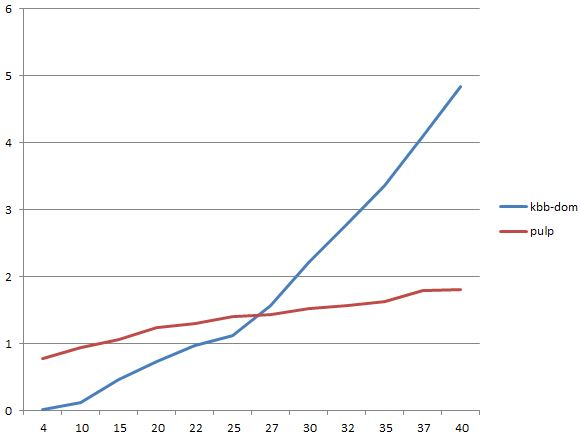
\includegraphics[scale=0.6]{1}
\end{center}
\caption{Comparison of KBB and pulp \label{numfig}}
\end{figure}

As we can see from the Table \ref{numtab} and Figure \ref{numfig}, KBB algorithm is faster than Pulp in small instances, but seems to be rather difficult to solve larger instance. This result is different from what is recored in \cite{fukasawa2011exact}, which says KBB always outperforms PuLP, no matter how large the instance is. There are two possible reasons to this difference. First, KBB is a problem-specific algorithm, which solves complicated integer knapsack problem. However, the instances we have are only binary integer knapsack problems, which are more simple instances. Solving these instances may lose the advantage of KBB. When we emailed Dr. Goycoolea, we asked him whether he could provide us those instances he used, but got no response for this request. Second, our implementation can be improved, probability in branch and bound algorithm. Since we don't know what specific technique that the auther used in his implementation, we only adopt Depth-First-Search strategy, the criteria by which to select the node down which to dive was not clear. We guess the latter reason is the main one to cause this difference between our implenmentation and the original one.

Second, we try to figure out what it is that makes KBB work so much better than PuLP,  we show first that part of this difference comes from the pre-processing. In this part, due to the difficulty of finding the appropriate instances, we randomly generate some more general integer knapsack instances of dimension from 4 to 50. For problems in each dimension, we generate 10 instances.  All the weight vectors and cost vectors have integer entries from -100 to 100. We compare the number of variables before and after preprocessing, computing time as following.

\begin{table}[H]
\begin{center}
\begin{tabular}{l c c c c c c c c}
\hline
nvar&4&10&15&20&25&30&40&50\\
\hline
nppvar &2&4.9 &8.1 &10.2 &12.4 &14.5 &18.7 &26.2\\
time&0.004&0.033&0.245&0.493&0.988&1.503&2.936&4.706\\
pptime&0.014&0.027&0.078&0.169&0.381&0.469&1.168&2.986\\
pulptime&0.342&0.403&0.457&0.514&0.557&0.599&0.686&0.702\\
pppulptime&-&-&0.397&0.431&0.483&0.482&0.503&0.612\\
\hline
\end{tabular}
\end{center}
\caption{The effectiveness of preprocessor \label{t3}}
\end{table}

In table \ref{t3}, $nvar$ represents the number of variables before preprocessing, $nppvar$ represents the average number of variables after preprocessing.  We find an interesting things, the average number of variables always reduces around half after preprocessing. The reason of this might be that this 6 steps preprocessing procedure we mentioned in section 2(!!!!!!!reasons!!!!!!!), which leads to half of the variables become reduntant after step 3. 

\begin{figure}[H]
\begin{center}
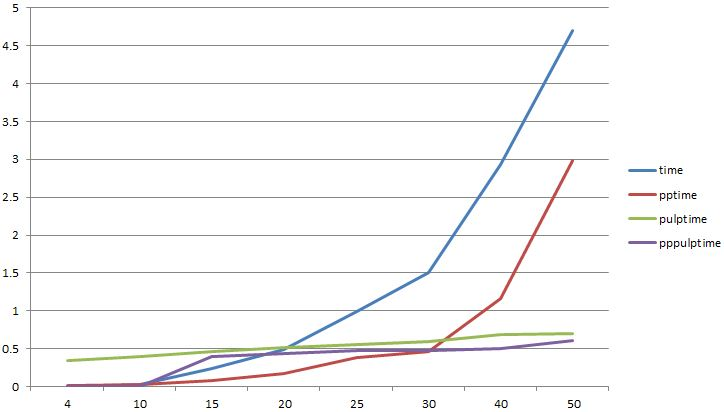
\includegraphics[scale=0.6]{3}
\end{center}
\caption{The effectiveness of preprocessor: computing time \label{numfigp}}
\end{figure}

In terms of computing time, $time$ means the computing time for KBB algorithm without preprocessing procedure to solve instances,  while $pptime$ means the the computing time of KBB algorithm with preprocessing. $pulptime$ and $pppulptime$ represent the time of PuLP algorithm without and with preprocessing respectively. However, when the number of variables are 4 and 10, it throws out Error if we use this preprocessor on PuLP, which is surprising. We find that this preprocessor has more impact on KBB algorithm than PuLP algorithm. This is not surprising, perhaps, if we consider that CPLEX already counts with its own, very effective set of pre-processing routines. On the more difficult instances preprocessor provides much time reduction which is also as our expectation..

Then, we show that under the same pre-processing, what will happen if we didn't use domination based braching strategy. Table \ref{t4} and Figure \ref{f3} give us the comparison of computing time between PuLP, KBB with domination and KBB without domination, represented by pulp, kbb-dom and kbb-no-dom.

\begin{table}[H]
\begin{center}
\begin{tabular}{l c c c c c c}
\hline
nvar&4&10&15&20&22&25\\
\hline
kbb-no-dom&0.014&0.198&0.685&1.242&1.497 &1.647\\
kbb-dom&0.009&0.116&0.468&0.737&0.966&1.118\\
pulp&0.779&0.940&1.060&1.234&1.297&1.398\\
\hline\hline
nvar&27&30&32&35&37&40\\
\hline
kbb-no-dom&2.051&2.353&2.919&3.493&4.012&4.550\\
kbb-dom&1.576&2.129&2.776&3.357&4.095&4.835\\
pulp&1.430&1.519&1.565&1.628&1.788&1.813\\
\hline
\end{tabular}
\end{center}
\caption{Comparison of KBB and pulp\label{t4}}
\end{table}

\begin{figure}[H]
\begin{center}
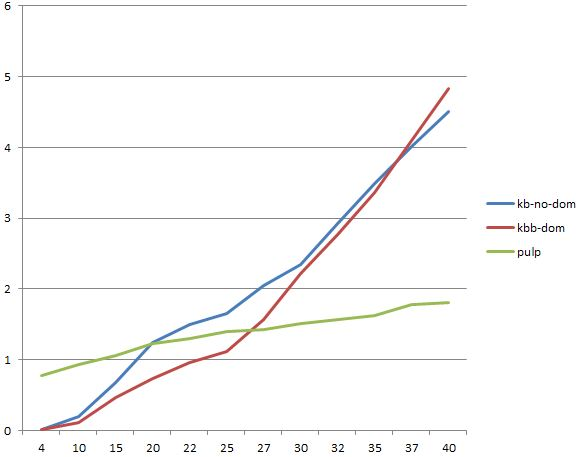
\includegraphics[scale=0.6]{2}
\end{center}
\caption{Comparison of KBB and pulp \label{f3}}
\end{figure}

This comparison shows the effectiveness of domination stategy also depends on the dimension of instances. When the instances have small number of variables, domination strategy may lead to a huge improvement to KBB algorithm. However, as the dimension of problems grows, the time gap between KBB with domination and KBB without domination strategy becomes smaller and smaller. Then dealing with instances with 37 and 40 variables, it is even faster if we give up domination, which is different from what was recorded by Goycoolea.

Again, the problem seems come from the implementation. Domination strategy uses a large number of iterations to get a tigher bound. This number of iterations dramatically increases with the number of variables in our implementation, which can be hardly improved by us. Thus, even though the tighter bound leads to the less iterations in branch and bound, the cost of which also cannot be ignored. However, as in \cite{fukasawa2011exact}, domination has a greater chance to result in an improvement, which means that there should be some ways to improve our implentation to domination algorithm.

Finally, we change the parameter $branch direction$ to see what happens. As in our first experiment shows, we adopt a Depth-First-Search strategy, but the criteria by which to select the node down which to dive was not clear. Here we set parameter $branch direction$ to be $up$ and $down$. The instances we consider here are also randomly generateed instances whose dimension is 30. 

\begin{table}[H]
\begin{center}
\begin{tabular}{l c c }
\hline
 & up & down\\
\hline
ave-time&1.923 & 2.219\\
ave-bbnodes& 61039& 662831\\
\hline
\end{tabular}
\end{center}
\caption{different $brach direction$\label{t5}}
\end{table}

Table \ref{t5} shows the average time and average nodes that visited for different strategies. We find the two diving strategies performed similarly well when considering the entire test set. This does not mean, however, that the instances performed similarly well on a one-to-one basis. In fact, it was observed that some particular instances were very sensitive to the diving strategy employed. This is partially reflected in Table \ref{t5} where it can be seen how the average time and the average number of visited nodes varied with the diving strategies.



\section{Summary}
In this project, We implemented the algorithm in \cite{fukasawa2011exact}. With seven subroutine algorithms and a main function. We list the function of these seven functions as following
\begin{itemize}
\item By introducing the definition of efficiency, the first algorithm show us it the original is infeasible ,unbounded or trivial solution. In our code, it named pre-processing.
\item After the first step, if we detected that the original problem is not trivial, then we further use a simple eight-step pre-processing procedure in order to reduce an instance of MIKP to another, equivalent
instance of MIKP, so called PP-MIKP which is easier to solve.
\item We then focus on solving the LP relaxation of PP-MIKP which derived from the second step. First we the algorithm to solve a so-called Primal phase I algorithm, which can verify whether an instance is infeasible or obtain $x$, a $k$-efficient solutions with non-negative slack.
\item Move on to this so-called primal phase II algorithm, which takes the $k$-efficient solution from the primal phase I algorithm and supply an optimal solution to the LP relaxation problem or show the infeasibility of the LP relaxation problem .
\item We can also use dual phase II algorithm to derive the optimal solution or the LP relaxation or show if this problem is infeasible.
\item Next a branching algorithm is provided, which is a easy way to avoid solving the new LP relaxation of PP-MIKP to optimality from scratch. By using the down direction and upper direction, we update activity and objective, and then choose primal phase II or dual phase II to resolve the problem.
\item The last algorithm is what we used to speed up the branching and improve the bound, including cost-Domination, lexicographic-Domination. Furthermore, by using the domination, we improve the branch and bound algorithm, by building a domination table. 
\end{itemize}

After implementing it, we conducted extensive computational experiments. We aim to reproduce the improvement brought by the new algorithm KBB
brings in \cite{fukasawa2011exact}. In the practical test, we use 549 binary knapsack instances to derive the numerical results, because we can't find the same instance the author used in their numerical experiment. What's more, instead of comparing the KBB algorithm with Cplex solver, our algorithm is the comparison with KBB algorithm and Pulp solver. Implemented in python, we showed that the KBB is more efficient than pulp when solving the small size problem, However, when solving the large size problem, the efficiency decreased. We assume the difference comes from the language we used, since in \cite{fukasawa2011exact}, the authors implement algorithm in C++.  After this, we generated some random problem and further show the performance of pre-processing and simplification of our algorithm and stated all the result in the table \ref{numtab} and figure \ref{numfigp}. At last, we show the importance of domination that is used to improve the efficiency of branch and bound algorithm.

\textbf{Acknowledgments} We appreciate professor Goycoolea for his explanation of our problems on implementation of these algorithms and some information that he supplied for better understand of domination.  

\newpage
\bibliographystyle{plain} 
\bibliography{literature}
 
\end{document}
